% At tree level, there are three contributions to the $\PW^+\PW^+$ production in association with two jets: the pure EW component $\mathcal{O}(\alpha^6)$, the interference $\mathcal{O}(\alphas\alpha^5)$, and the QCD background $\mathcal{O}(\alphas^2\alpha^4)$
% \AK{We have mentioned this many times at this point. Perhaps not worth repeating again?}.
In the present section, the cross sections and distributions are obtained without applying the VBS cuts on the variables $m_{\Pj\Pj}$ and $|\Delta y_{\Pj\Pj}|$, 
Eq.~(\ref{cut:4}).
In Tab.~\ref{tab:LOscanXsec}, the cross sections of the three LO contributions are reported.
The EW, QCD, and interference contributions amount to $57\%$, $37\%$, and $6\%$ of the total inclusive cross section, respectively.
The QCD contribution does not posses external gluons due to charge conservation.
Thus the diagrams of order $\mathcal{O}(g_{\rm s}^2g^4)$ only involve gluon exchange in the $t/u$-channel between the quark lines.
This results in a small contribution even if the VBS cuts have not been imposed.
The interference between EW and QCD contributions is small, due to color suppression, but not negligible.
% ($t/u$ and $t/s$ interferences with identical fermions).

\begin{table}[h!]
    \centering
    \begin{tabular}{c|c|c|c}
        Order & $\mathcal{O}(\alpha^6)$ & $\mathcal{O}(\alphas^2\alpha^4)$ & $\mathcal{O}(\alphas\alpha^5)$ \\
        \hline
        \hline
        $\sigma[\rm{fb}]$ & $ 2.292 \pm 0.002 $ & $ 1.477 \pm 0.001 $ & $ 0.223 \pm 0.003 $ \\
%         {\sc Xxx}&  $ \pm $ & $ \pm $ & $ \pm $
    \end{tabular}
    \caption{\label{tab:LOscanXsec} Cross sections at LO accuracy for the three contributions to the process ${\rm p}{\rm p}\to\mu^+\nu_\mu{\rm e}^+\nu_{\rm e}{\rm j}{\rm j}$, obtained with exact matrix elements.
    These results are for the set-up described in Sec.~\ref{subsec:inputpar} but no cuts on $m_{\Pj\Pj}$ and $|\Delta y_{\Pj\Pj}|$ are applied.
    The uncertainties shown refer to the estimated statistical error of the Monte Carlo programs.}
\end{table}

In Fig.~\ref{fig:mjjdyjj_1d} these three contributions are shown separately and summed in the differential distributions in the di-jet invariant mass $m_{\Pj\Pj}$ and the rapidity difference $|\Delta y_{\Pj\Pj}|$.
For the di-jet invariant-mass  distribution (left), one can observe that the EW contribution peaks around an invariant mass of about $80\GeV$.
This is due to diagrams where the two jets originate from the decay of a W boson (see middle and right diagrams in Fig.~\ref{diag:LO}).
Note that these contributions are not present in calculations relying on the VBS approximation.
The EW contribution becomes dominant for di-jet invariant mass larger than $500\GeV$.
The same holds true for jet-rapidity difference larger than $2.5$ (right).
This justifies why cuts on these two observables are used in order to enhance the EW contribution over the QCD one.
In particular, in order to have a large EW contribution, rather exclusive cuts are required.

\begin{figure*}[hbt]
\centering
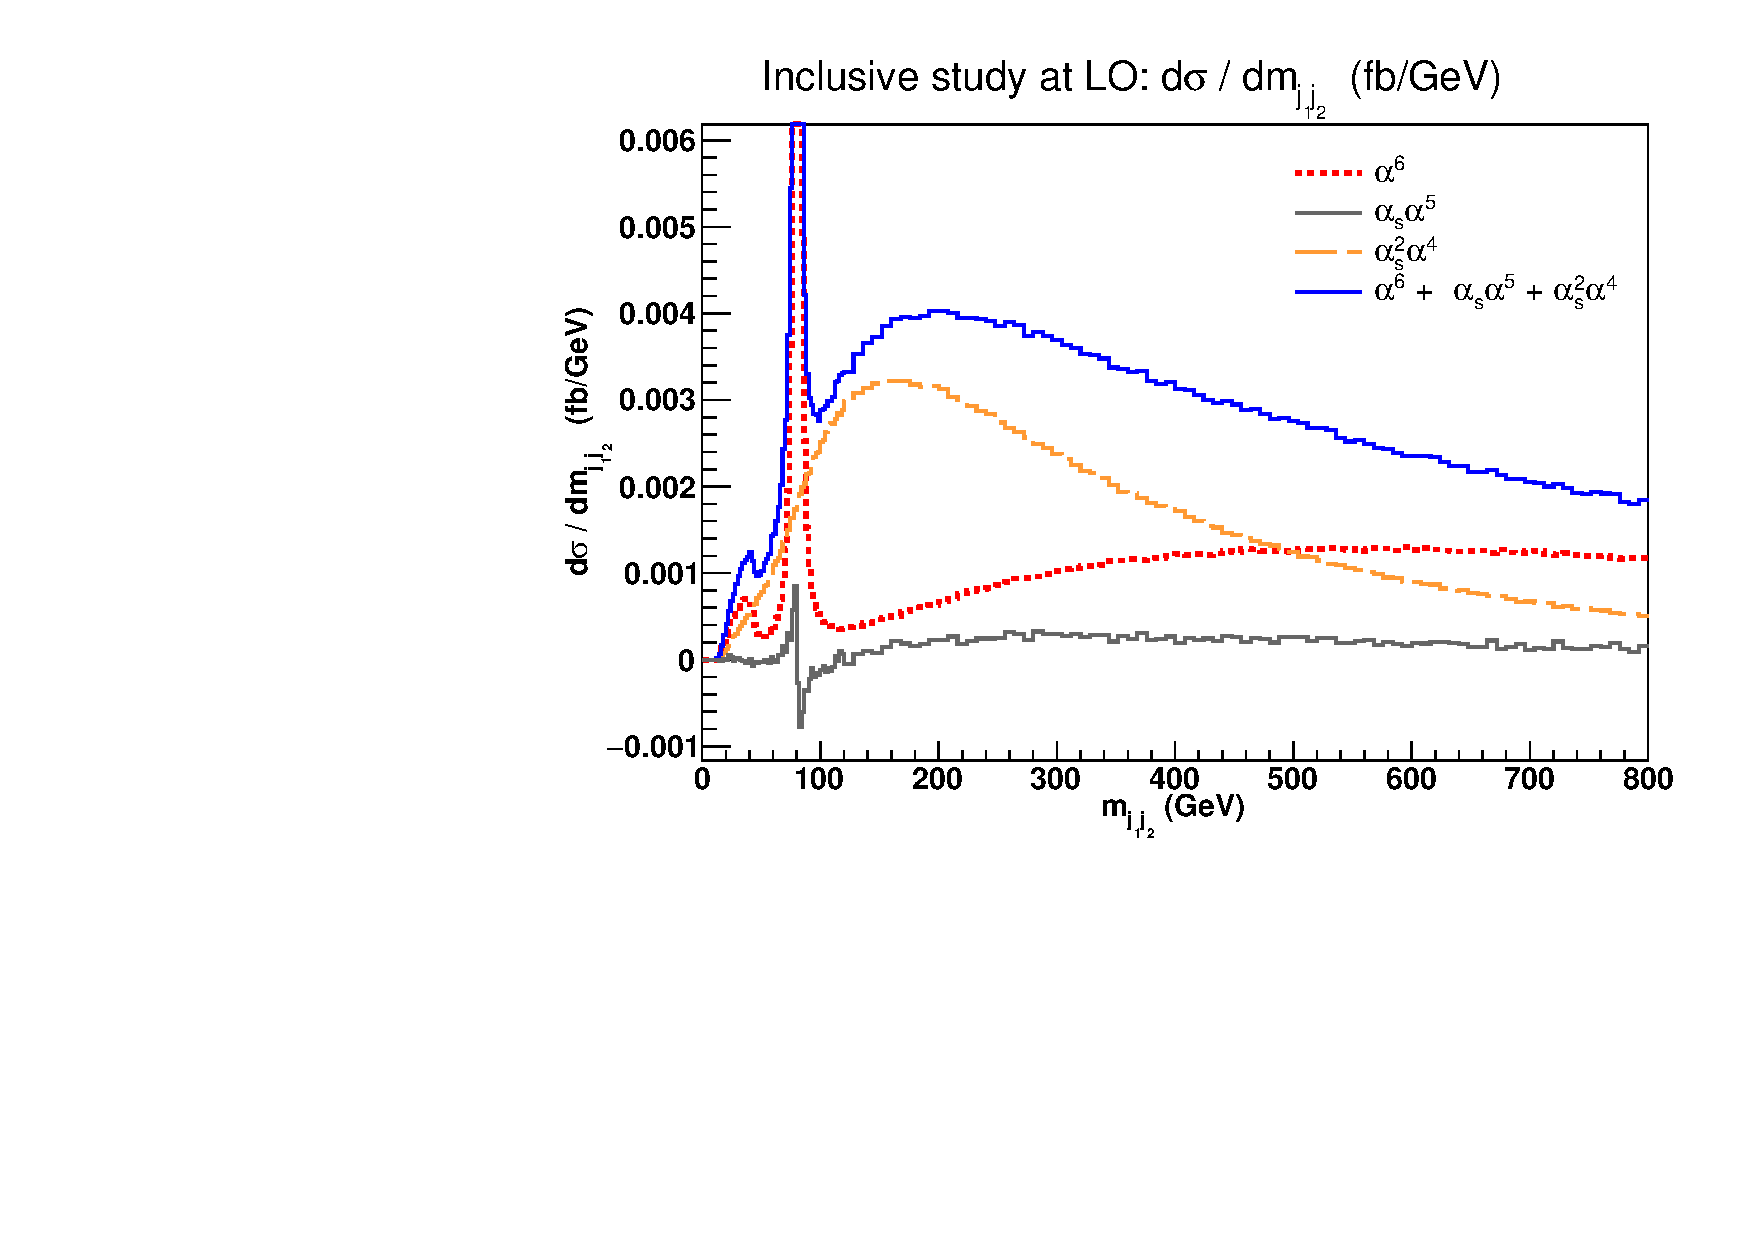
\includegraphics[scale=0.395]{figures/scanfigures/mjj_full.pdf}
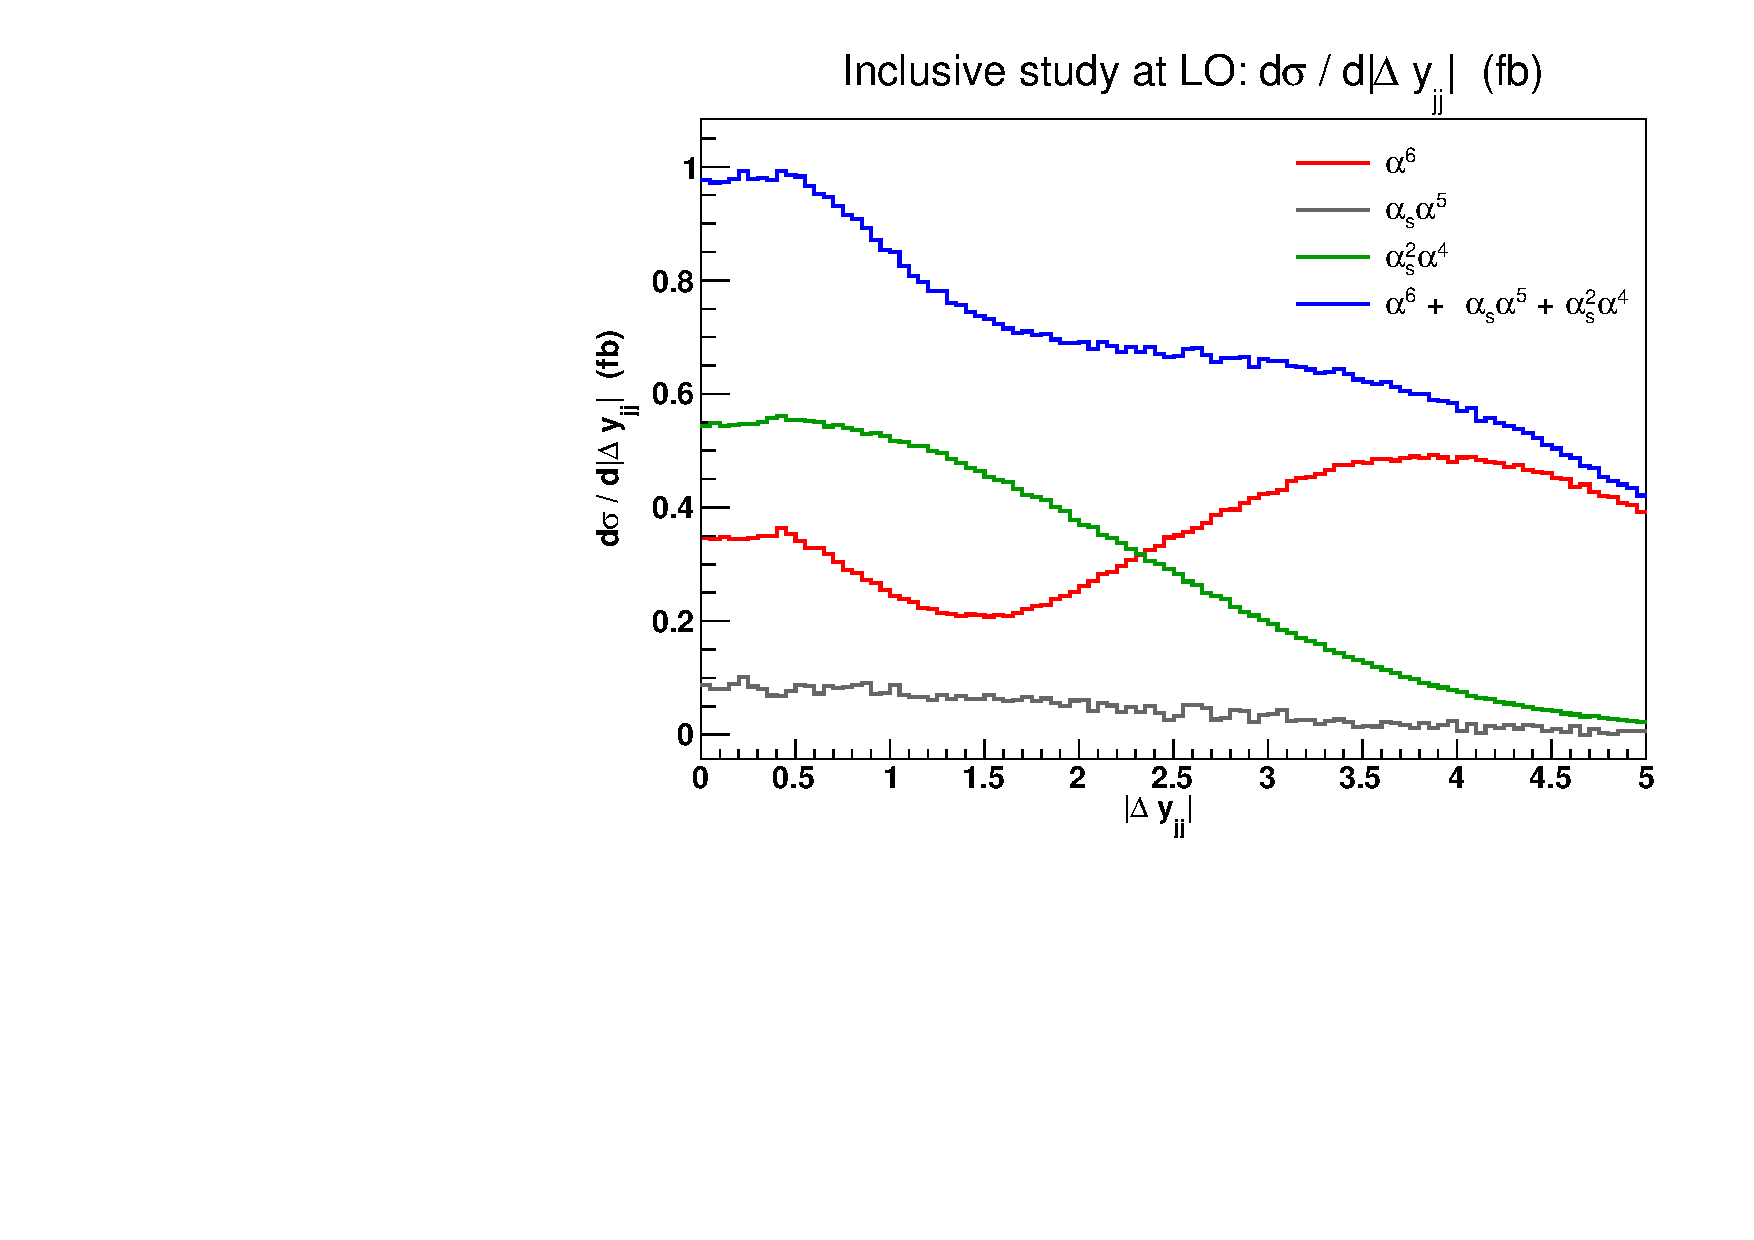
\includegraphics[scale=0.395]{figures/scanfigures/dyjj_full.pdf}
\caption{Differential distribution in the di-jet invariant mass $m_{\Pj\Pj}$ (left) and the difference of the jet rapidities $|\Delta y_{\Pj\Pj}|$ (right) for the three LO contributions to the process ${\rm p}{\rm p}\to\mu^+\nu_\mu{\rm e}^+\nu_{\rm e}{\rm j}{\rm j}$.
The EW contribution is in red, the QCD one in green, and the interference one in grey.
The sum of all the contributions is in blue.
The cuts applied are the ones of Sec.~\ref{subsec:inputpar} but no cuts on $m_{\Pj\Pj}$ and $|\Delta y_{\Pj\Pj}|$ are applied.}
\label{fig:mjjdyjj_1d}
\end{figure*}

This can also be seen in Fig.~\ref{fig:mjjdyjj_2d_LO} where the three contributions are displayed as double-differential distributions in the di-jet invariant mass and jet rapidity difference.
Again, it is clear that the region with low di-jet invariant mass should be avoided in VBS studies as it is dominated by tri-boson contributions.
% This motivates in particular the choice of $m_{\Pj\Pj} > 200\GeV$ and $|\Delta y_{\Pj\Pj}| > 2$ for our inclusive study (see below).
%Finally, let us notice that the choice $m_{\Pj\Pj} > 500\GeV$ and $|\Delta y_{\Pj\Pj}| > 2.5$ made by the experimental collaborations is well motivated in order to enhance the EW contribution over its irreducible backgrounds.
This motivates in particular the choice of employing the cut $m_{\Pj\Pj} > 200\GeV$ for our LO inclusive study in Sec.~\ref{subsec:LOinclusive}.

\begin{figure*}[hbt]
\centering
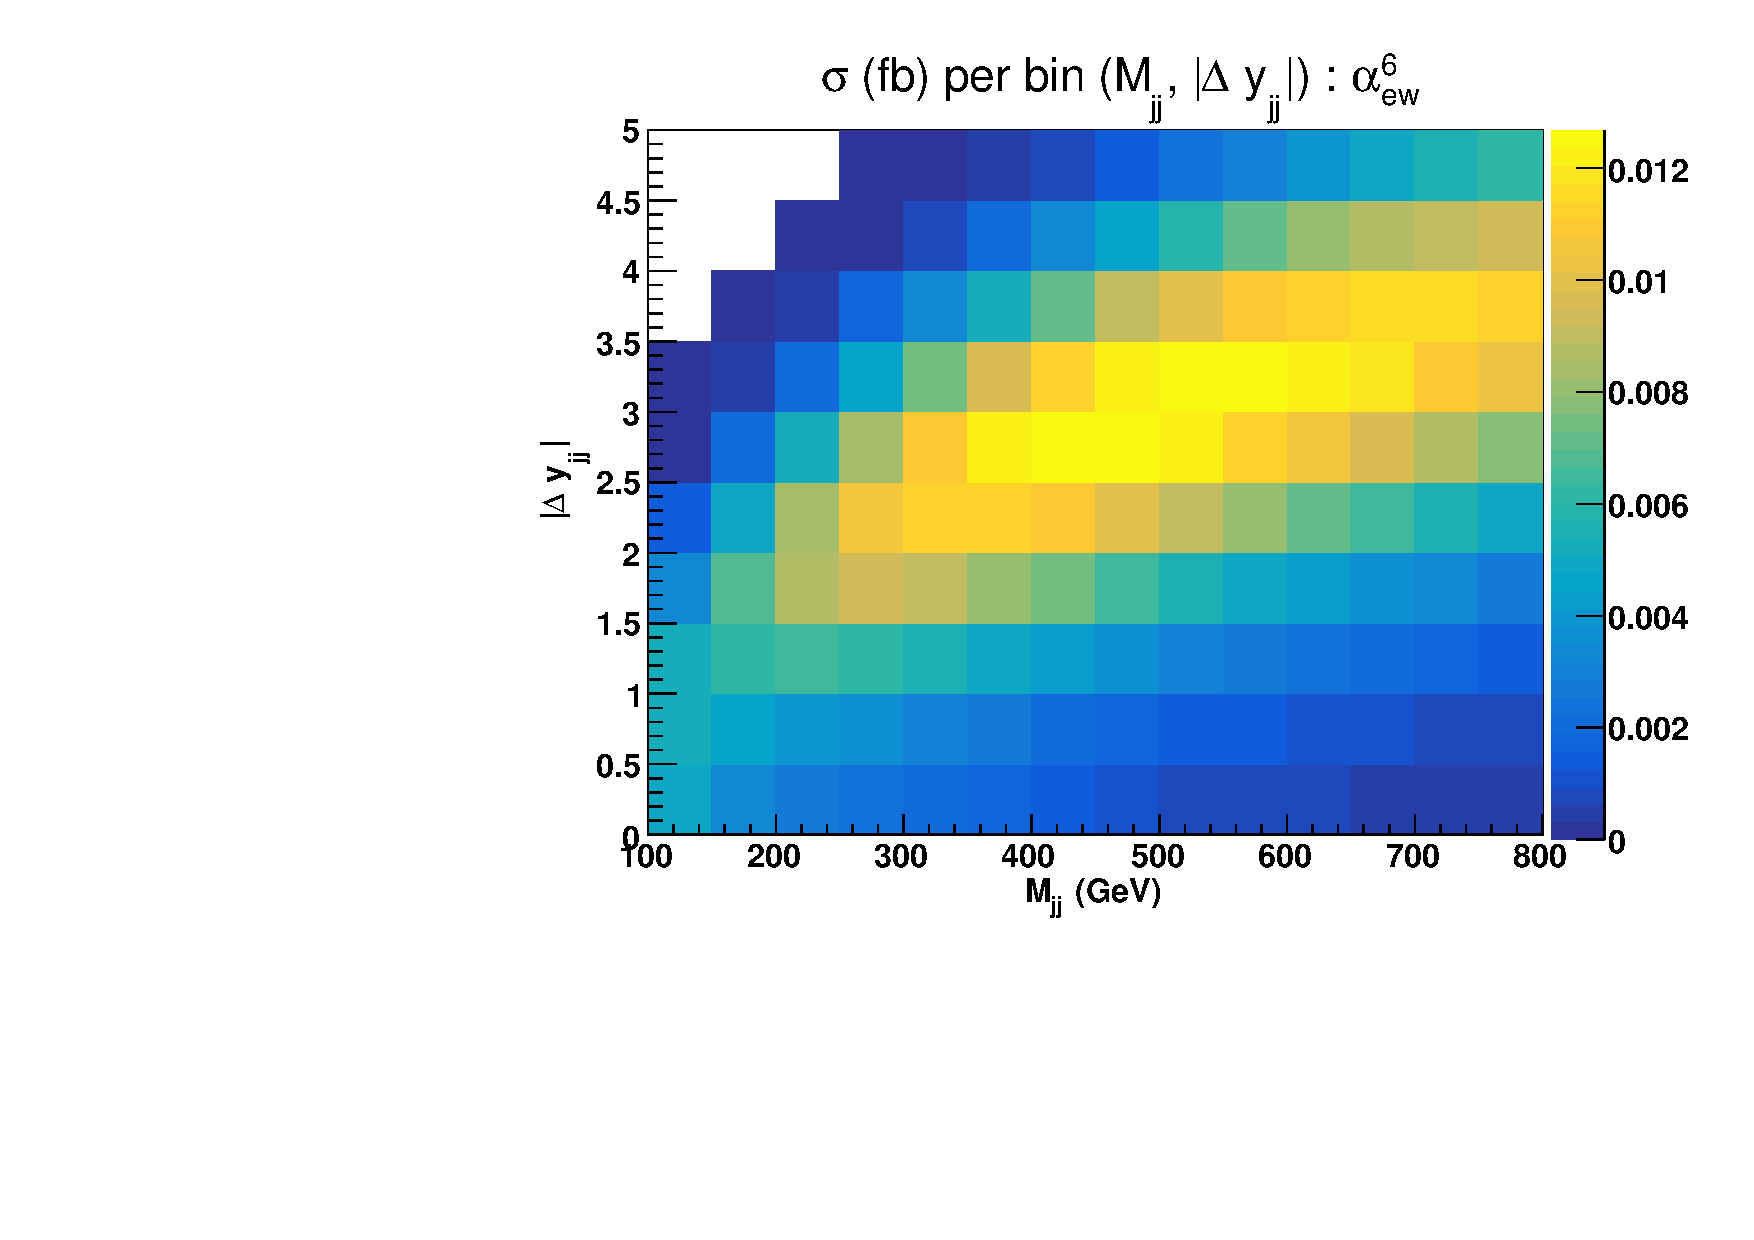
\includegraphics[scale=0.395]{figures/scanfigures/scan_ew6.pdf}
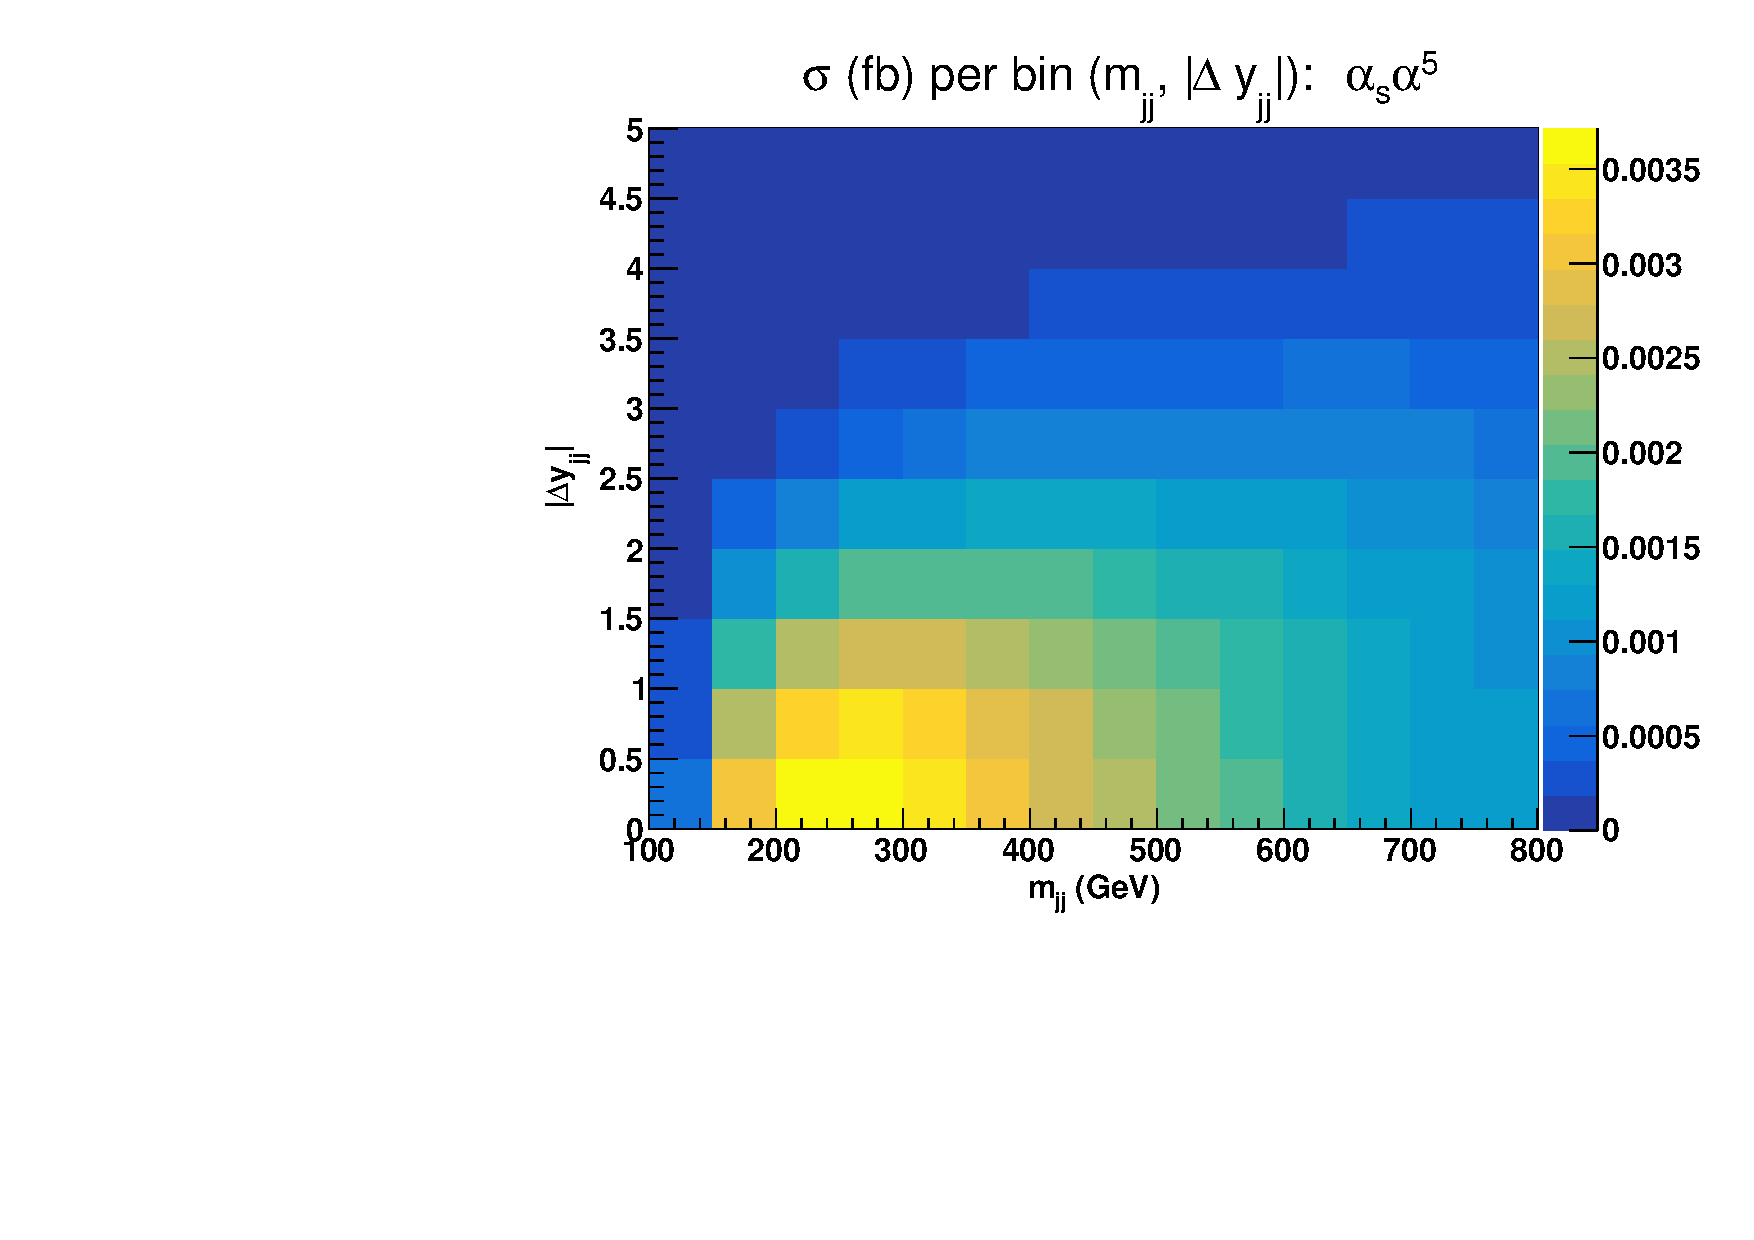
\includegraphics[scale=0.395]{figures/scanfigures/scan_ew5qcd1.pdf}
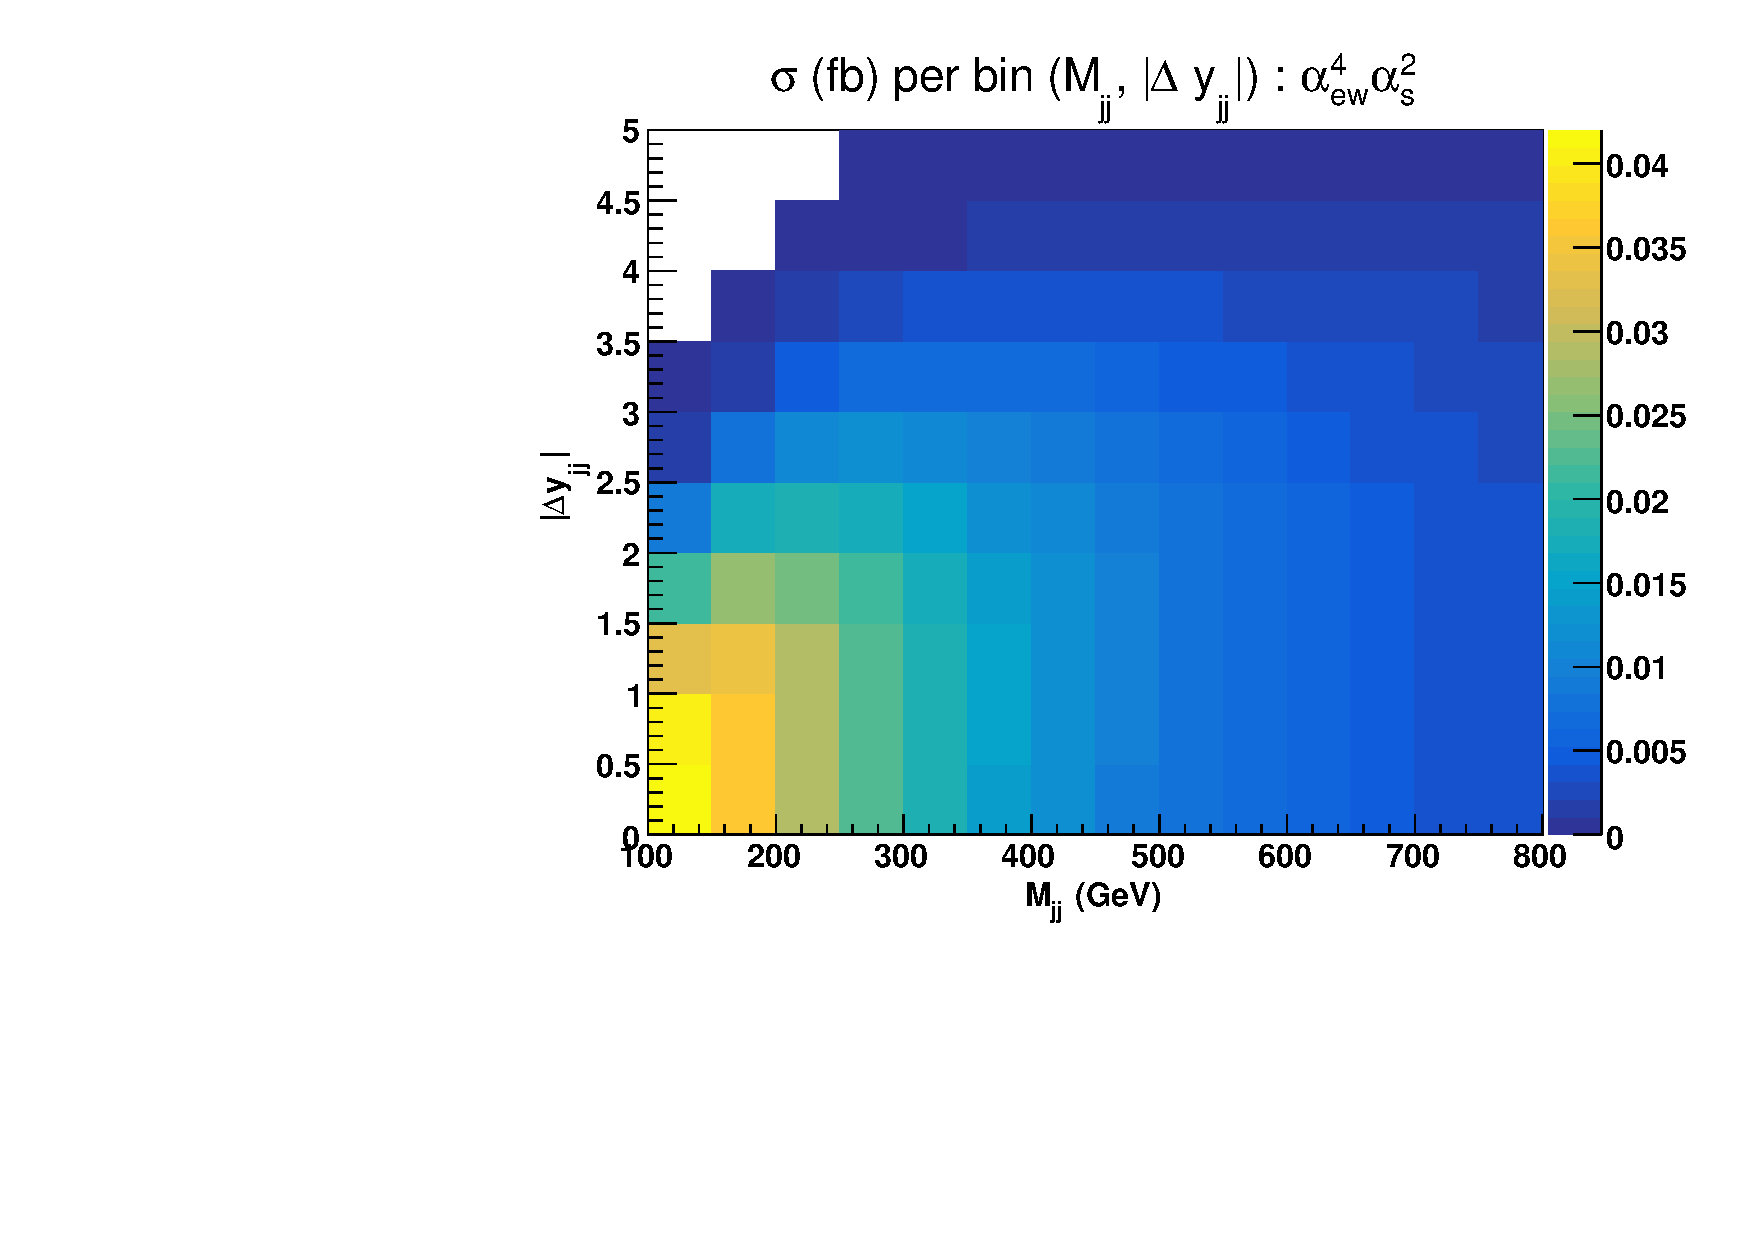
\includegraphics[scale=0.395]{figures/scanfigures/scan_ew4qcd2.pdf}
\caption{Double-differential distributions in the variables $m_{\Pj\Pj}$ and $|\Delta y_{\Pj\Pj}|$ for the three LO contributions of orders $\mathcal{O}(\alpha^6)$ (top left), $\mathcal{O}(\alphas\alpha^5)$ (top right), and $\mathcal{O}(\alphas^2 \alpha^4)$ (bottom).
The cuts applied are the ones of Sec.~\ref{subsec:inputpar} but no cuts on $m_{\Pj\Pj}$ and $|\Delta y_{\Pj\Pj}|$ are applied.
}
\label{fig:mjjdyjj_2d_LO}
\end{figure*}
